\chapter{序論}
\label{introduction}
本章では本研究の背景とモチベーション,および全体の構成について記述する.

\section{IPv6シングルスタックネットワークに求められる役割}
\label{introduction:background}

\subsection{IDCネットワークを取り巻く環境}
\subsubsection{IDC市場の広がり}
% 単純にIDC事業が伸びていることを言う.


近年,ライブ映像配信のようなリアルタイムなサービスに対するニーズが年々高まっている.例えばCisco社の調査\cite{index2017global}によれば,2022年には全てのアプリケーショントラフィックのうちインターネットビデオが有する割合が82%を超え,そのうち17%がライブ映像配信が占めると予想されている.
リアルタイムな高品質サービスを提供するためには,ユーザーの地理的に近いサービス拠点から配信を行うことが有効であるため,今後IDC・コンテンツ事業者が各地域拠点を介したコンテンツ配信基盤を活用するしていくことが予想される.

% 災害リスクから拠点を増やしたい話
一方で,インフラストラクチャに対する災害や地政学的リスクの軽減は,コンテンツ事業者の継続的な事業の成長のためには避けては通れない課題である\cite{alonso2001business}.
2011年に発生した東日本大震災以降,国内のIDC事業者やコンテンツ事業者を中心に,関東大都市圏に集中していたサービス拠点への依存性を解消するために,東京圏以外の各地域にサービス拠点を分散する取り組みが活発だ\cite{JANOG44_robust}.大阪・名古屋の他の都市圏のIDCは2019年現在満床状態が続いているほか,他の地方拠点都市も含めたIDC建設も並行して行われている. 

特に近年ではVXLANやSRv6のような新しいネットワーク仮想化技術の標準化も進み,サービス拠点のマルチテナンシーと柔軟性を両立するネットワークデザインの障壁が低くなってきているため,今後より多くのIDC・コンテンツ事業者のサービス拠点の拡大が続くと想定できる.


\subsubsection{IPv4アドレスの枯渇}
\label{introduction:background:ipv4_problems}
2019年現在,IANA\footnote{Internet Assigned Numbers Authority.インターネットに利用される様々な資源を一元的に管理する組織.\url{https://www.iana.org/}}が保有するIPv4アドレスプールは既に枯渇しており\cite{IANA_allocation},各RIR\footnote{Regional Internet Registry.}からも2021年頃までには新規割当が行えなくなることが予想されている\cite{potaroo_IPv4}.

\begin{figure}
	\centering
	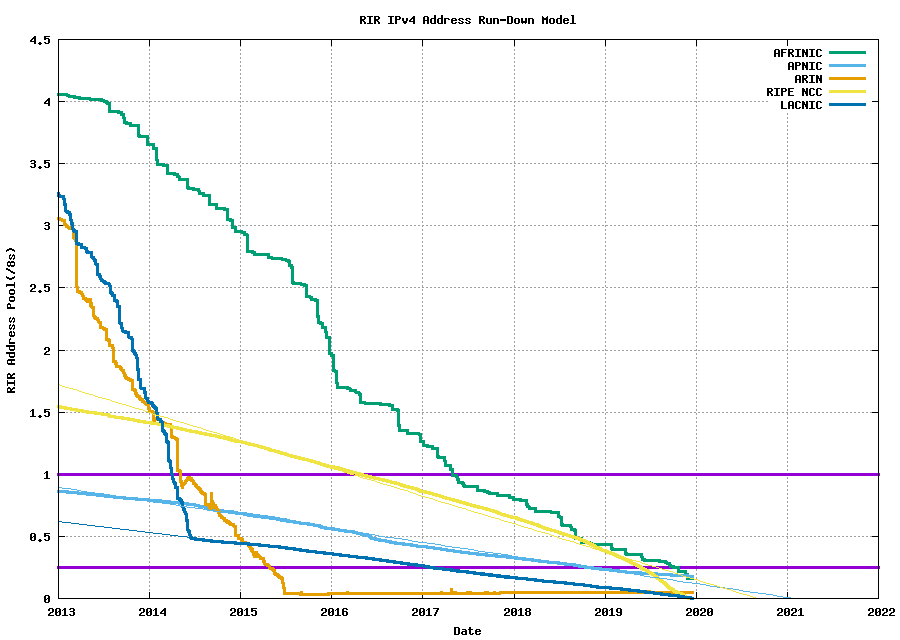
\includegraphics[width=8cm]{img/plotend.png}
	\caption{Projection of consumption of Remaining RIR Address Pools. \url{potaroo.net}より引用\cite{potaroo_IPv4}}
	\label{potaroo_IPv4_fig}
\end{figure}
    
一方で近年は民間事業者間アドレス取引も盛んに行われている.一般に新規にIPv4アドレスの割当を受けるためにはこのような民間取引市場を利用する方法が考えられるが,1アドレスあたりの単価は年々上昇傾向にあり\cite{howard2013internet},新規にIPv4ネットワークを構築するためのコストは日々上昇していくことが考えられる.




\subsubsection{IPv4/IPv6デュアルスタックネットワークの問題}
\label{introduction:background:dualstack_problems}
IPv6プロトコルの導入に主に用いられていた手法としてIPv4/IPv6デュアルスタックネットワークが挙げられる\cite{durand2001deploying}.IPv4/IPv6デュアルスタックネットワークとは,IPv4ネットワークとIPv6ネットワークを同一機器群上に並行して運用する手法であり,企業・一般家庭向けアクセスネットワークを中心にIPv4/IPv6デュアルスタック環境の整備が進んでいる.

一方でコンテンツ事業者が運用するIDCでは以下の主な3つの理由からデュアルスタック環境の導入はデメリットが大きい.

\begin{itemize}
    \item \textbf{IPv4アドレスの継続的調達が困難} \\
    先に述べたように,IPv4アドレスをサービスの成長にあわせて継続的に調達していくことは困難である.民間市場の市況に調達コストが左右されるため長期的な見通しが立てにくい.
    \item \textbf{オペレーションコストの肥大化}\\
デュアルスタック環境では2つの異なるIPプロトコルを同時に運用する必要があるため、シングルスタック環境と比べて運用コストの上昇が見込まれる\cite{北口善明2017クライアント}.
    
    \item \textbf{ネットワーク機器の性能要件の上昇}\\
デュアルスタック環境では,シングルスタック環境よりも多くの経路をネットワーク機器が保持しなければならないため,より高性能な機器を導入する必要がある.
\end{itemize}



\subsection{IPv6シングルスタックネットワーク}
\label{introduction:background:IPv6-single-stack-network}
IDC事業者・コンテンツ事業者がビジネスを健全に拡大するためには,IPv6ネットワークのみで機器間を接続したIPv6シングルスタックネットワークの利用が不可欠である.

IDCのIPv6シングルスタックネットワークには以下のような働きが期待される.


\subsubsection{IPv4サービスの提供}
Google社が定常的に行っている調査\cite{Google_IPv6_statistics}によれば,2019年12月現在全世界のインターネットトラフィックの7割程度をIPv4トラフィックが依然として占めている.

コンテンツ事業者のIPv6シングルスタックネットワークにおいても何らかの手段を用いてIPv4サービスを継続して提供する必要がある.

\subsubsection{シングルスタック運用によるOPEX/CAPEXの削減}
第\ref{introduction:background:dualstack_problems}項で述べたように,IPv4/IPv6デュアルスタックネットワークではオペレーションコストの肥大化が問題視されていた.
IPv6シングルスタックネットワークではIPv4ネットワークを廃止することが出来るため,OPEX\footnote{Operating expense. 運用に掛かる継続的なコスト.}とCAPEX\footnote{Capital expenditure. 設備配備に掛かる初期投資コスト.}の軽減が期待される.

\subsubsection{IPv4/IPv6デュアルスタックネットワークと同等以上の性能}
IPv6により提供されるサービスはもちろんのこと,IPv4によるサービスにおいてもIPv4/IPv6デュアルスタックネットワークと同等の耐障害性・サービス品質・サービス容量が保証されることが望ましい.

とりわけネイティブなIPv4ネットワーク以外の手段を用いて提供されるIPv4サービスの性能の担保が運用課題になると予想される.




\section{本研究のモチベーションと取り組み}

第\ref{introduction:background:IPv6-single-stack-network}項で述べたようなIPv6シングルスタックネットワークに求められる要件のうち,IPv4サービスの提供における冗長性や構成変更への追従性の向上を促す手法の確立を目指す.

本研究ではIPv6シングルスタックネットワークにおけるIPv4サービスの提供手法のうち,アーキテクチャがシンプルで広範な利活用が期待されるSIIT-DC\cite{RFC7755}に着目した.
SIIT-DCとはIPv6ネットワークとIPv4ネットワークの各境界部に,BR\footnote{Border Relay.IP/ICMP変換アルゴリズムのステートレスモード\cite{RFC7915}を実装した機器.}を配備することにより,IPv6ネットワークのみに属するホストで仮想的にIPv4サービスを提供するネットワーク設計を定めたインターネット標準である.SIIT-DCにおいて各BRは静的に定義されたアドレス変換テーブルを利用してネットワークプロトコル変換を行うため,BRを複数配備する場合における一貫性の確保や冗長性,IDC内の構成変更に対する追従性の面で課題があった.

本研究では動的経路アルゴリズムの一つであるBGP\cite{RFC4271}を利用したメッセージングによるアドレス変換テーブルの動的な広告手法を提案する.
エミュレータを利用した概念実証実験により,本提案手法がこれらの課題に対して効果的に作用することが証明された.



\section{本論文の構成}

本論文の構成を以下に示す.

~\ref{background}章では,背景を述べる.
~\ref{issue}章では,本研究における問題の定義と,解決するための要件の整理を行う.
~\ref{proposed}章では,本研究の提案手法を述べる.
~\ref{implementation}章では,~\ref{proposed}章で述べたシステムの実装について述べる.
~\ref{evaluation}章では,\ref{issue}章で求められた課題に対しての評価を行い,考察する.
~\ref{conclusion}章では,本研究のまとめと今後の課題についてまとめる.


%%% Local Variables:
%%% mode: japanese-latex
%%% TeX-master: "../thesis"
%%% End:
